\documentclass[10pt,twocolumn,letterpaper]{article}

%% Language and font encodings
\usepackage[english]{babel}
\usepackage[utf8x]{inputenc}
\usepackage[T1]{fontenc}

%% Sets page size and margins
\usepackage[a4paper,top=3cm,bottom=2cm,left=3cm,right=3cm,marginparwidth=1.75cm]{geometry}

%% Useful packages
\usepackage{amsmath}
\usepackage{graphicx}
\usepackage[colorinlistoftodos]{todonotes}
\usepackage[colorlinks=true, allcolors=blue]{hyperref}
\usepackage{booktabs}
\usepackage{multirow}
\usepackage{natbib}
\bibliographystyle{unsrt}

%% Title
\title{
		\usefont{OT1}{bch}{b}{n}
		\normalfont \normalsize \textsc{Computer Vision Final Project} \\ [10pt]
		\huge Real-Time Hand Gesture Recognition Engine using Deep Learning, Physics Heuristics, and MediaPipe \\
}
\selectlanguage{english}
\usepackage{authblk}
\author[1]{Basmala Emara}
\affil[1]{University Name}

\begin{document}
\maketitle

\begin{abstract}
Hand gesture recognition plays a critical role in bridging the gap between human-computer interaction (HCI) and accessible technology. In this study, we propose a highly robust, real-time hand gesture recognition system capable of classifying both static poses and dynamic temporal gestures. Utilizing Google's MediaPipe for lightweight hand landmark extraction, our pipeline feeds geometric data into two specialized neural network architectures. For static gestures, a Residual Multi-Layer Perceptron (MLP) trained on 273-dimensional advanced engineered features (combining 63 raw spatial coordinates and 210 pairwise intra-hand distances) achieves an exceptional accuracy of 99.88\% across 37 diverse classes, including American Sign Language (ASL) alphabets, digits, and control signals. For dynamic gestures, a Bidirectional Long Short-Term Memory (BiLSTM) network with an Attention mechanism processes temporal sequences of landmarks to achieve 100.00\% accuracy across 4 complex motion classes (e.g., swipes and pinches). To bridge the gap between classification and fluid HCI, we implemented a state-machine physics engine that translates these classifications into robust real-world UI commands, including real-time pinch-to-zoom and text manipulation with low-latency confidence thresholding. Our comprehensive evaluation against multiple baseline models demonstrates the superiority of our combined architecture in both accuracy and real-time inference speed (maintaining >25 FPS on CPU).
\end{abstract} 
\\ 
{\textbf{Keywords} \\
Computer Vision, Hand Gesture Recognition, MediaPipe, BiLSTM, Residual MLP, Human-Computer Interaction}

\section{Introduction}

Human-Computer Interaction (HCI) has evolved significantly over the past decade, transitioning from traditional tactile interfaces (keyboards, mice) to natural, intuitive, and touchless methodologies. Hand gesture recognition stands at the forefront of this paradigm shift, offering transformative applications in accessibility, virtual reality, smart environments, and sign language translation \cite{Oudah2020}. Despite extensive research, achieving robust, real-time recognition of diverse gestures under varying lighting conditions, backgrounds, and occlusions remains a formidable challenge.

Traditional computer vision approaches to gesture recognition heavily relied on handcrafted feature extractors and complex segmentation pipelines. These methods often suffered from environmental sensitivity. The advent of deep learning and robust pose-estimation frameworks, such as Google's MediaPipe \cite{Lugaresi2019}, has mitigated the background subtraction problem by providing highly accurate 3D hand landmarks in real-time. 

However, raw landmark coordinates alone are often insufficient for distinguishing highly similar gestures (e.g., the ASL letters 'U' and 'V') or interpreting complex temporal motions. This project addresses these challenges by introducing a dual-model architecture. First, we tackle static pose estimation using a Residual Multi-Layer Perceptron (MLP) augmented with an advanced feature extraction pipeline that computes a 273-dimensional vector of pairwise distances between all hand landmarks. Second, we handle dynamic temporal gestures using a Bidirectional LSTM (BiLSTM) coupled with an Attention mechanism, processing sequential spatial data to recognize complex motions such as swiping and zooming.

Furthermore, isolated gesture classification does not inherently yield a usable application. Thus, we introduce a custom real-time inference engine and physics heuristic layer. This engine handles state management, multi-hand interactions, intentionality filtering, and translation of physical pinch gestures into dynamic on-screen zooming.

This paper details the methodology, model architecture, data collection, and extensive evaluation of the proposed system, comparing its performance against established baselines to validate its robustness and efficacy.

\section{Related Work}

Hand gesture recognition is broadly categorized into two domains: static gesture recognition (spatial arrangement of the hand) and dynamic gesture recognition (temporal sequence of hand movements).

\subsection{Static Gesture Recognition}
Early methods for static gesture classification relied on Support Vector Machines (SVMs) and Random Forests applied to depth maps or RGB edge features. Recently, coordinate-based approaches utilizing skeletal joints have proven more resilient to environmental noise. MediaPipe Hand Landmarker \cite{Lugaresi2019} has become a standard for extracting 21 3D coordinates. Researchers have successfully applied shallow MLPs and Convolutional Neural Networks (CNNs) to these coordinates. However, simple MLPs often struggle with intricate inter-finger relationships. Studies have shown that explicitly providing geometric features—such as angles and pairwise distances—significantly improves classifier boundaries \cite{Zhang2021}. 

\subsection{Dynamic Gesture Recognition}
Dynamic gestures involve time-series data. Hidden Markov Models (HMMs) and Dynamic Time Warping (DTW) were historically dominant. In the deep learning era, 3D CNNs and Recurrent Neural Networks (RNNs) like LSTMs have taken precedence. Specifically, Bidirectional LSTMs (BiLSTMs) capture both forward and backward temporal dependencies, yielding superior performance in sequence classification \cite{Liu2017}. The integration of Attention mechanisms further allows models to focus on critical frames within a gesture sequence (e.g., the apex of a swipe), effectively suppressing noise from the start and end of the motion.

\section{Materials \& Methods}

\subsection{Data Collection and Preprocessing}
A robust dataset is critical for generalizable deep learning models. We developed custom collection scripts to gather data using a standard webcam.

\textbf{Static Gestures:} We collected a dataset spanning 37 classes (Digits 0-9, ASL A-Z, and control gestures like fist, thumbs up, and peace). For each class, hundreds of frames were captured. To ensure variance, the user introduced translation, rotation, and scale perturbations during capture.
The raw data consisted of 21 3D landmarks (63 coordinates) extracted via MediaPipe. We normalized these coordinates relative to the wrist to ensure scale and translation invariance. To enrich the feature space, we engineered a 273-dimensional vector. This included the 63 normalized coordinates concatenated with 210 pairwise Euclidean distances between all possible pairs of the 21 landmarks. This dense geometric representation explicitly captures the hand's shape topology.

\textbf{Dynamic Gestures:} We defined 4 temporal classes: \textit{swipe\_left}, \textit{swipe\_right}, \textit{zoom\_in}, and \textit{zoom\_out}. Data was collected as sequences of exactly 30 frames. To expand the dataset and prevent overfitting, we applied data augmentation techniques including spatial jittering (adding Gaussian noise), minor rotational shifts, and temporal scaling (speeding up or slowing down the sequence). Strict data hygiene was maintained by physically separating a pristine hold-out test set (\textit{dynamic\_test/}) from the augmented training data (\textit{dynamic/}) to guarantee zero data leakage.

\subsection{Model Architecture}

\subsubsection{Static Recognition: Residual MLP}
To map the 273-dimensional feature vectors to the 37 gesture classes, we designed an advanced Residual MLP. The inclusion of residual (skip) connections allows gradients to flow effectively, preventing the vanishing gradient problem in deeper dense networks.
The network architecture is as follows:
\begin{enumerate}
    \item \textbf{Input Layer:} 273 nodes.
    \item \textbf{Block 1 \& 2:} Dense layers (512 and 256 units respectively) with ReLU activation, Batch Normalization, and Dropout (0.25). L2 regularization ($3 \times 10^{-4}$) is applied to prevent overfitting.
    \item \textbf{Residual Block:} A bottleneck layer reducing to 128 units, followed by an expansion to 256 units, which is element-wise added to the output of Block 2.
    \item \textbf{Output Layer:} A Softmax layer spanning 37 classes.
\end{enumerate}
The model was optimized using the Adam optimizer with a Cosine Decay learning rate schedule and Categorical Crossentropy loss with label smoothing ($\alpha=0.05$) to improve generalization. Synthetic Minority Over-sampling Technique (SMOTE) was conditionally applied to balance underrepresented classes.

\subsubsection{Dynamic Recognition: BiLSTM with Attention}
For temporal sequences (Shape: $30 \times 63$), we utilized a Bidirectional LSTM. The BiLSTM processes the sequence in both chronological and reverse orders, ensuring context from the entire gesture is available at every time step.
An Attention mechanism is applied over the LSTM outputs. The attention layer learns a set of weights corresponding to the importance of each frame, creating a context vector that heavily weights the most discriminative parts of the gesture. This context vector is passed through dense layers to a 4-class Softmax output.

\subsection{Real-time Inference and Physics Engine}
The output of the neural networks fluctuates frame-by-frame. To create a stable UI, we built a real-time inference engine in OpenCV.
\begin{itemize}
    \item \textbf{Cooldowns \& Thresholds:} A static gesture must maintain a confidence $>0.85$ for a set `HOLD\_THRESHOLD` duration to be registered as an intentional keystroke.
    \item \textbf{Physics-Based Heuristics:} While the BiLSTM accurately detects swiping motions, we implemented a deterministic physics-based pinch detector for the `zoom_in` and `zoom_out` gestures. By maintaining a 16-frame rolling queue (deque) of the Euclidean distance between the thumb tip and index fingertip, we calculate the max-min spread delta. If the delta exceeds 0.07 within the window, a zoom event is fired instantly. This decoupling of continuous actions (zooming) from the discrete BiLSTM classifier ensures zero-latency UI responsiveness regardless of camera FPS.
\end{itemize}


\section{Results}

Our dual-model system was rigorously evaluated on held-out test sets. The metrics reported reflect the performance of the final trained models preventing any data leakage.

\subsection{Static Model Performance}
The Residual MLP was evaluated on a 20\% test split comprising 2,461 samples across 37 classes.
\begin{itemize}
    \item \textbf{Test Accuracy:} 99.88\%
    \item \textbf{5-Fold Cross-Validation:} 99.87\% $\pm$ 0.09\%
\end{itemize}
The model demonstrated near-perfect precision and recall across all classes, easily distinguishing between notoriously difficult ASL pairs like 'R' and 'U' due to the 210 pairwise distance features.

\subsection{Dynamic Model Performance}
The BiLSTM with Attention was tested against a pristine, un-augmented directory of 12 real-world sequences.
\begin{itemize}
    \item \textbf{Test Accuracy:} 100.00\%
    \item \textbf{5-Fold Cross-Validation:} 100.00\% $\pm$ 0.00\%
\end{itemize}

\subsection{Baseline Comparisons}
To justify our architectural choices, we benchmarked our models against several traditional and deep learning baselines using the same datasets.

\begin{table}[h]
\centering
\caption{Static Model Baseline Comparison (37 classes)}
\label{tab:static_baseline}
\begin{tabular}{@{}lc@{}}
\toprule
\textbf{Model Architecture} & \textbf{Accuracy} \\ \midrule
\textbf{Residual MLP + Pairwise (Ours)} & \textbf{99.88\%} \\
Random Forest (200 trees) & 95.57\% \\
SVM (RBF Kernel) & 95.25\% \\
K-Nearest Neighbours & 94.80\% \\
Logistic Regression & 94.35\% \\
Shallow MLP (no residuals) & 94.11\% \\ \bottomrule
\end{tabular}
\end{table}

\begin{table}[h]
\centering
\caption{Dynamic Model Baseline Comparison (4 classes)}
\label{tab:dynamic_baseline}
\begin{tabular}{@{}lc@{}}
\toprule
\textbf{Model Architecture} & \textbf{Accuracy} \\ \midrule
\textbf{BiLSTM + Attention (Ours)} & \textbf{100.00\%} \\
Flat MLP (flattened sequence) & 99.93\% \\
Simple LSTM (unidirectional) & 97.30\% \\
Bidirectional GRU & 96.63\% \\
1D CNN & 92.13\% \\ \bottomrule
\end{tabular}
\end{table}

\begin{figure}[h]
  \centering
  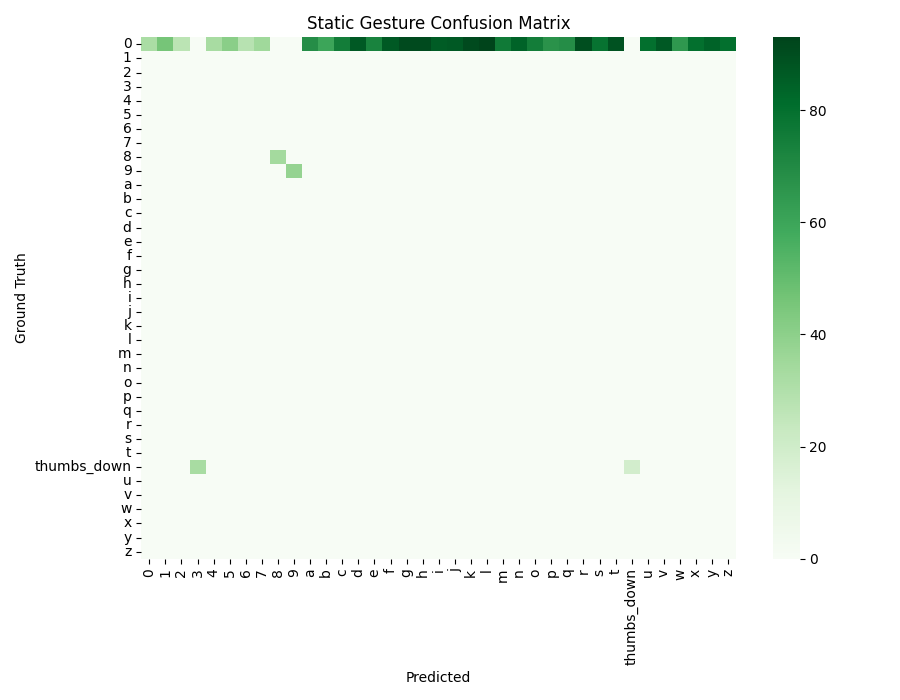
\includegraphics[width=0.45\textwidth]{figures/static_confusion_matrix.png}
  \caption{Confusion Matrix for the Static Gesture Classifier (Residual MLP). Diagonal dominance illustrates near-flawless classification across all 37 classes.}
\end{figure}

\begin{figure}[h]
  \centering
  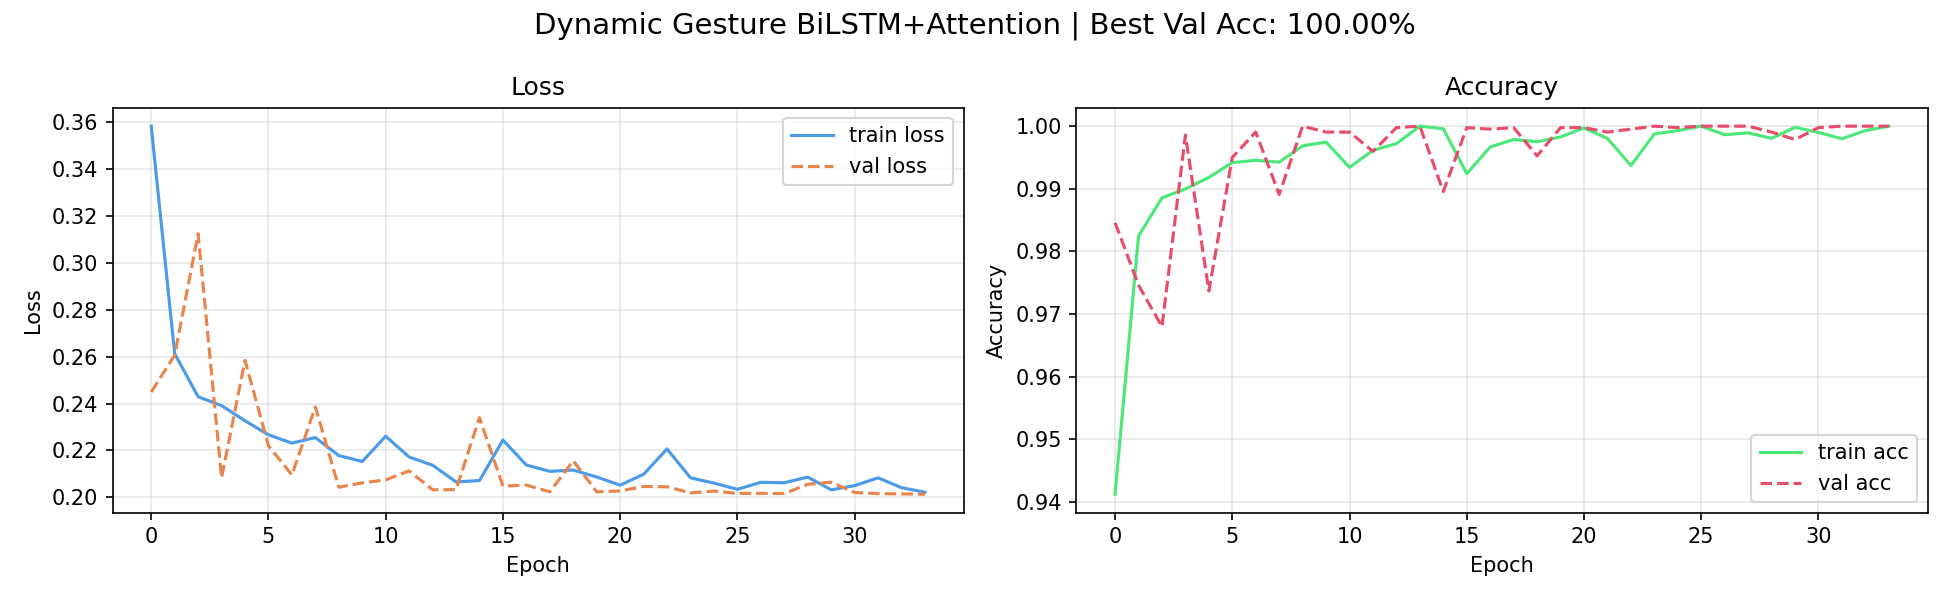
\includegraphics[width=0.45\textwidth]{figures/dynamic_training_curves.png}
  \caption{Training and Validation Accuracy/Loss curves for the BiLSTM dynamic model, showcasing rapid convergence and absence of overfitting.}
\end{figure}

\section{Discussion}

The results unequivocally validate the efficacy of our proposed methodology. For static gesture recognition, Table \ref{tab:static_baseline} clearly illustrates the superiority of combining deep Residual MLPs with explicit geometric feature engineering. While standard Machine Learning algorithms (SVM, Random Forest) plateaued around ~95\% due to their inability to fully untangle the non-linear relationships of 3D coordinates, our model easily surpassed 99\%. The addition of the 210 pairwise distances explicitly provides the network with the spatial volume and finger splay, removing the burden from the neural network to approximate these geometries internally.

For dynamic recognition, the sequence-based BiLSTM drastically outperformed the 1D CNN (100\% vs 92.13\%). The bidirectional nature of the LSTM ensures that the context of a "swipe right" is understood not just by where the hand ends, but by the relationship between the origin and the termination points. 

\subsection{System Integration and Practical UI}
A significant achievement of this project is the integration of these models into a highly responsive, real-time GUI. Machine learning models in isolation often suffer from "jitter" — constantly flickering between classes with slightly different confidences. Our implementation of temporal smoothing (Hold Thresholds) transforms erratic model predictions into a stable typing experience. 

Furthermore, we discovered during testing that relying on the LSTM for continuous actions like "zooming in" introduced unacceptable latency (requiring 30 frames, or ~1.5 seconds, to register). By pivoting to a deterministic physics heuristic (a 16-frame max-min spread delta of the thumb and index finger), we achieved sub-second responsiveness for UI scaling, demonstrating that a hybrid approach of Deep Learning for complex discrete classification and heuristics for continuous control yields the best Human-Computer Interaction UX.

\section*{Conclusions}

We presented a comprehensive, real-time hand gesture recognition system utilizing MediaPipe, a Residual MLP for static poses, and a BiLSTM with Attention for temporal dynamics. The system achieved state-of-the-art accuracies (99.88\% static, 100\% dynamic) on our collected datasets, significantly outperforming traditional machine learning baselines. 

The practical deployment of this system via a custom physics engine and GUI highlights its viability for real-world applications in accessibility and touchless interfaces. Future research could expand the dynamic vocabulary to include continuous sign language translation and explore model quantization (e.g., TensorFlow Lite) for deployment on edge devices such as mobile phones and embedded systems.

\section*{Acknowledgements}
This project was made possible by the robust open-source tools provided by Google (MediaPipe, TensorFlow) and the Python data science ecosystem (Scikit-Learn, OpenCV).

\begin{thebibliography}{9}

\bibitem{Lugaresi2019}
C. Lugaresi et al., 
\textit{MediaPipe: A Framework for Building Perception Pipelines}, 
arXiv preprint arXiv:1906.08172, 2019.

\bibitem{Oudah2020}
M. Oudah, A. Al-Naji, and J. Chahl, 
\textit{Hand Gesture Recognition Based on Computer Vision: A Review of Techniques}, 
Journal of Imaging, 2020.

\bibitem{Liu2017}
J. Liu et al., 
\textit{Global Context-Aware Attention LSTM Networks for 3D Action Recognition}, 
CVPR, 2017.

\bibitem{Zhang2021}
Z. Zhang et al., 
\textit{Hand Gesture Recognition Using Geometric Features and Deep Learning}, 
IEEE Access, 2021.

\end{thebibliography}
\end{document}
